%!Cau!%
\begin{ex}%[Thi thử L1, Chuyên Nguyễn Trãi, Hải Dương, 2019]%[Đinh Thanh Hoàng, dự án EX6]%[1D1K1-2]
	\immini{
		Cho hàm số $f(x)$ có đồ thị như hình bên. Hàm số $g(x)=\ln \left(f(x)\right)$ đồng biến trên khoảng nào dưới đây?
		\choice
		{$(-\infty;0)$}
		{\True $(1;+\infty)$}
		{$(-1;1)$}
		{$(0;+\infty)$}
	}{
		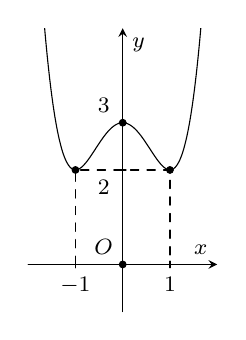
\begin{tikzpicture}[scale=0.6, font=\footnotesize, line join=round, line cap=round, >=stealth]
			\draw[->] (-2,0)--(2,0) node[above left]{\footnotesize $x$};
			\draw[->] (0,-1)--(0,5) node[below right] {\footnotesize $y$};
			\foreach \x in {-1,1}	\draw[shift={(\x,0)},color=black] (0pt,2pt) -- (0pt,-2pt) node[below] {\footnotesize $\x$};
			\foreach \y in {3}		\draw[shift={(0,\y)},color=black] (2pt,0pt) -- (-2pt,0pt) node[above left] {\footnotesize $\y$};
			\foreach \y in {2}		\draw[shift={(0,\y)},color=black] (2pt,0pt) -- (-2pt,0pt) node[below left] {\footnotesize $\y$};
			\filldraw (0,0) circle(2pt) node [above left] {\footnotesize $O$};
			\filldraw (-1,2)circle(2pt) (0,3)circle(2pt) (1,2)circle(2pt);
			\begin{scope}
				\clip (-2,-1) rectangle (2,5);
				\draw[domain=-2:2,samples=100,smooth,variable=\x] plot (\x,{(\x)^4-2*(\x)^2+3});
			\end{scope}
			\draw[dashed] (-1,0)--(-1,2)--(1,2)--(1,0);
		\end{tikzpicture}
	}
	\loigiai{
		Ta có $g'(x)=\left[\ln \left(f(x)\right)\right]'=\dfrac{f'(x)}{f(x)}$.\\
		Từ đồ thị hàm số $y=f(x)$ ta thấy $f(x)>0$ với mọi $x\in \mathbb{R}$. Vì vậy dấu của $g'(x)$ là dấu của $f'(x)$. Ta có bảng biến thiên của hàm số $g(x)$
		\begin{center}
			\begin{tikzpicture}[scale=1, font=\footnotesize, line join=round, line cap=round, >=stealth]
				\tkzTabInit[nocadre=false,lgt=1.2,espcl=2.5,deltacl=0.6]
				{$x$ /0.6,$y'$ /0.6,$y$ /2}
				{$-\infty$,$-1$,$0$,$1$,$+\infty$}
				\tkzTabLine{,-,$0$,+,$0$,-,$0$,+,}
				\tkzTabVar{+/ $+\infty$ ,-/,+/,-/,+/$+\infty$}
			\end{tikzpicture}
		\end{center}
		Vậy hàm số $g(x)=\ln \left(f(x)\right)$ đồng biến trên khoảng $(1;+\infty)$.
	}
\end{ex}%!Cau!%
\begin{ex}%[Thi thử L1, Chuyên Bến Tre, 2019]%[Lê Quốc Hiệp,12EX-9-2019]%[1D1K1-5]
	Tìm tất cả các giá trị thực của tham số $m$ sao cho $\sin^3 x+\cos^3 x\le m$ với mọi $x\in\mathbb{R}$.
	\choice
	{\True $m\ge1$}
	{$m=1$}
	{$m\le1$}
	{$-1\le m\le1$}
	\loigiai
	{
		Ta có $\heva{&\sin x\le1\\&\cos x\le1}\Rightarrow\heva{&\sin^3 x\le\sin^2 x\\&\cos^3x\le\cos^2x.}$\\
		Như vậy $\sin^3 x+\cos^3 x\le1$ (Dấu ``='' xảy ra khi $x=k2\pi$ hoặc $x=\dfrac{\pi}{2}+k2\pi$,~$k\in\mathbb{Z}$).\\
		Khi đó $\sin^3 x+\cos^3 x\le m$ với mọi $x\in\mathbb{R}$ khi và chỉ khi $m\ge1$.
	}
\end{ex}